\documentclass[onecolumn, draftclsnofoot,10pt, compsoc]{IEEEtran}
\usepackage{graphicx}
\usepackage{url}
\usepackage{setspace}
\usepackage{csquotes}
\usepackage{float}
\usepackage{soul}
\usepackage{color}
\usepackage{pstricks-add}

\usepackage{listings}
\RequirePackage{pgfcalendar}
\usepackage{pgfgantt}
\usepackage{pdflscape}
\usepackage{tikz}


% COLOR DEFINITIONS FOR CODE LISTINGS
\definecolor{codegreen}{rgb}{0,0.6,0}
\definecolor{codegray}{rgb}{0.5,0.5,0.5}
\definecolor{codepurple}{rgb}{0.58,0,0.82}
\definecolor{backcolour}{rgb}{0.95,0.95,0.92}

\lstdefinestyle{mystyle}{
    backgroundcolor=\color{backcolour},
    commentstyle=\color{codegreen},
    keywordstyle=\color{magenta},
    numberstyle=\tiny\color{codegray},
    stringstyle=\color{codepurple},
    basicstyle=\footnotesize,
    breakatwhitespace=false,
    breaklines=true,
    captionpos=b,
    keepspaces=true,
    numbers=left,
    numbersep=5pt,
    showspaces=false,
    showstringspaces=false,
    showtabs=false,
    tabsize=2
}

\lstset{
	escapeinside={(*@}{@*)},
	style=mystyle
}

\usepackage{geometry}
\geometry{textheight=9.5in, textwidth=7in}

% 1. Fill in these details
\def \CapstoneTeamName{	Short Circuit Comedy Club	}
\def \CapstoneTeamNumber{		CS13}
\def \GroupMemberOne{			Kevin Talik}
\def \GroupMemberTwo{			Arthur Shing}
\def \GroupMemberThree{			Anish Asrani}
\def \CapstoneProjectName{		How to Build an Effective Robot Comedian}
\def \CapstoneSponsorCompany{	Oregon State University}
\def \CapstoneSponsorPerson{		Dr. Heather Knight}

% 2. Uncomment the appropriate line below so that the document type works
\def \DocType{		%Problem Statement
				%Requirements Document
				%Technology Review
				%Design Document
				Final Document
				}

\newcommand{\NameSigPair}[1]{\par
\makebox[2.75in][r]{#1} \hfil 	\makebox[3.25in]{\makebox[2.25in]{\hrulefill} \hfill		\makebox[.75in]{\hrulefill}}
\par\vspace{-12pt} \textit{\tiny\noindent
\makebox[2.75in]{} \hfil		\makebox[3.25in]{\makebox[2.25in][r]{Signature} \hfill	\makebox[.75in][r]{Date}}}}
% 3. If the document is not to be signed, uncomment the RENEWcommand below
%\renewcommand{\NameSigPair}[1]{#1}

%%%%%%%%%%%%%%%%%%%%%%%%%%%%%%%%%%%%%%%
\begin{document}
\begin{titlepage}
    \pagenumbering{gobble}
    \begin{singlespace}
 %   	\includegraphics[height=4cm]{coe_v_spot1}
        \hfill
        % 4. If you have a logo, use this includegraphics command to put it on the coversheet.
        %\includegraphics[height=4cm]{CompanyLogo}
        \par\vspace{.2in}
        \centering
        \scshape{
            \huge CS Capstone \DocType \par
            {\large\today}\par
            \vspace{.5in}
            \textbf{\Huge\CapstoneProjectName}\par
            \vfill
            {\large Prepared for}\par
            \Huge \CapstoneSponsorCompany\par
            \vspace{5pt}
            {\large Prepared by }\par
            Group\CapstoneTeamNumber\par
            % 5. comment out the line below this one if you do not wish to name your team
            \CapstoneTeamName\par
            \vspace{5pt}
            \vspace{20pt}
        }
        \begin{abstract}
  	     % 6. Fill in your abstract
			The purpose of this document is to outline the research papers that this team will create to conclude during Spring Term 2018.
			The three members of the \textit{Short Circut Comedy Club} have spent their time during winter term perfomring research under Dr. Heather Knight at Oregon State University.
			The focus of this project is to study the effect a robot comedian can have on a crowd of humans.
			Kevin Talik's research has been spent understanding what a Comedian can do to "Adapt" to a performance.
			Arthur Shing has been studying the voice of the robot, and the difference between "Robot and Human" character.
			One final aspect of Stand-Up Comedy that we studied is "Crowd Work". Anish Asrani has spent most of his time developing spontaneous Crowd-Interactions during the set.
        \end{abstract}
    \end{singlespace}
\end{titlepage}
\newpage
\pagenumbering{arabic}
\tableofcontents
% 7. uncomment this (if applicable). Consider adding a page break.
%\listoffigures
%\listoftables
\clearpage

\section{Introduction to Project}
Who requested it?
Why was it requested?
What is its importance?
Who was/were your client(s)?
Who are the members of your team?
What were their roles?
What was the role of the client(s)? (I.e., did they supervise only, or did they participate in doing development)

\section{Introduction - Requirements}
The field of human-robot interaction can learn a lot from stand-up comedy. A stand-up performance has a basis of scripted content, from which the comedian delivers jokes to engage the audience. Good Comedians can read the audience and sometimes adapt their delivery based on the mood of the room \cite{talkingFunny}. In social robotics, when a robot shares a space with a human, an interaction can influence the people's opinions of the robot. Additionally, evident character traits presented (through dialogue and non-verbal motion) by the machine can anthropomorphize itself, making it easier and more enjoyable to connect with for the human \cite{KnightEightLessons:2011}. The purpose of this work is to explicitly evaluate what aspects of a robot comedian's performance are most salient to human audience.


\section{Previous Research}

Research on the improvement of HRI is indispensable for our project. In Heather Knight's \textit{Eight Lessons}, gestures, liveliness, and joke timing are all aspects that can be incorporated into the robot {\cite{KnightEightLessons:2011}}.
Relatable and appropriate gestures significantly helps improve communication between the robot and the audience. If the actions are predictable, humans can relate to the robot.
When watching someone perform an action, the human brain maps the actions onto itself and simulates the action in the best way possible. This is a physiological experience that should be replicated by the robot in order to enhance relatability. Simplicity is important as well. {\cite{KnightEightLessons:2011}}

In addition, Knight observed that having the robot portrayed as a living character rather than just an object that is kept up on stage improved the overall experience for the observers. Having believable interactions can enhance the feeling of a living character.
The goal of the audience tracking using sensors is to maximize enjoyment. The enjoyment levels were be read by the robot and used to modify upcoming jokes {\cite{KnightEightLessons:2011}}. Pausing and letting the audience laugh is vital as well. Starting the next joke too early can break the rhythm and leave the audience baffled. Looking around and body poses should be used to fill the pause {\cite{KnightEightLessons:2011}}.

In a previous study of robot comedy \cite{RobotComedyLab:2015}, Katevas found that when a robot engaged the audience through eye contact, the audience was more receptive to the performance. Eye contact from the robot is important, as it is a non-verbal cue for direct interaction. The audience members can identify that the machine is making an attempt to engage with specific members of the audience. We will investigate this further by having the robot perform various non-verbal and verbal interactions using sensors. The idea is to have the audience be a part of the performance even if they are not the ones performing. This can be accomplished if the robot is socially intelligent.

Other studies by Katevas et al. \cite{KatevasRobot:2014} that involved evaluating the social dynamics of a live performance by a robot have used SHORE\textsuperscript{TM} vision framework software to analyze and detect faces in the audience. SHORE\textsuperscript{TM} allows for facial expression recognition, estimated age, gender, and eye or mouth openings \cite{SHORE}, giving the study a heterogeneous audience model. These allowed for the robot to interact directly with specific audience members. However, usage of SHORE\textsuperscript{TM} involves expenses and funds that are unavailable to us, so we will encounter behavioral limitations dealing with a homogeneous audience model.

A study by Guy Hoffman {\cite{hoffman2010anticipation}} noted the importance of anticipation in human-robot interaction (HRI). The timing and meshing of anticipatory action and perception are a useful framework for HRI. The greatest challenge when designing a robot that will perform on stage is to enable the robot to be both - expressive and responsive. Robot models in the past have ended up on either extreme; they are either real-time and do not allow for continuous expression, or they are very animated but do not allow well times reactive behavior.


Researchers have also proposed multiple design patterns to promote sociability in Human-Robot Interaction (HRI). Some of these include having an initial introduction, some sort of didactic communication, including personal interests or history, and recovering from mistakes \cite{Kahn:2008}. These patterns in design are proposed to allow for more effective and meaningful social interactions. While there is yet to be much data or research on the validity of these claims, they may still prove to be useful in guiding the designs of our project.


% The effectiveness of our robot comedian will be evaluated by human enjoyment levels. Specifics regarding measurements and analysis will be later discussed with the client. Some possible methods include handing out surveys for the audience to fill out, which may include questions regarding the subjective reception of the robot comedian. Additionally, behavioral statistics may be used to evaluate the effectiveness of the comedy.

Robots utilizing non-verbal communication and statically written audience engagement have been attempted in robot comedy. In particular, Knight has observed the importance of character and spontaneous interactions in creating effective comedy \cite{KnightEightLessons:2011}. However, there is little research on the actual effectiveness of character and spontaneous interactions \cite{KatevasRobot:2014}. This project will aim to examine the effectiveness of character and spontaneous interactions in robot comedy.

\section{Hypothesis}

Our research will be guided by the following questions:
\begin{enumerate}[\IEEEsetlabelwidth{6}]
\item How can the robot make the audience feel like a part of the performance?
\item How can the robot convey and a coherent and well-developed character?
\item How can the robot adapt and influence to the audience?
\end{enumerate}

We hypothesize that comedy scripts with greater degrees of (1) crowdwork, (2) character, and (3) adaptiveness, will create more effective comedy, and have a more positive response from the audience.

\subsection{Crowdwork}
% TODO: Explain why crowdwork might have effects (reference 8 lessons?) and what crowdwork might look like in a script

Keeping the audience engaged is vital in creating an entertaining performance. Katevas et al. had some success leading to a better audience response when using gestures and acknowledging the audience's presence. A successful performance manages the dynamics of various aspects of interaction to the benefit of both the performer and the audience \cite{RobotComedyLab:2015}. Interaction with the audience will make the comedian robot feel more authentic, like an entity, and less like an object. Knight's research found that the robot's connection with the audience is stronger if the robot is able to convey social intelligence. This helps the robot display that it is not just an inanimate object \cite {KnightEightLessons:2011}.

\subsection{Character}
% TODO: Find a better place to put this? Maybe it fits here
Expressing character will be understood from the robot under the "theory of the mind" \cite{leslie}. Understanding the agents meta-representation of a behavior is helpful for the audience in relating to the robot's intent, desires and knowledge. A robot attempts this to understand and relate its desires and intent better to the audience \cite{theoryOfMindRobots}.


% TODO: Explain why character might have effects (reference 8 lessons?) and what character might look like in a script
The appearance of character in a robot may create more effective comedy.
Research has shown that expressive behaviors in a robot may cause interacting humans to favor the robot \cite{DesignExBeh:2017}.
One could argue that expressive behaviors are behavioral actions formed by an inner character. While robots currently are not capable of having intrinsic character qualities, we postulate that a robot which behaves as if it has character could be more effective at engaging an audience. The task of conveying a sense of character may also benefit from social behaviors developed in researching the effectiveness of crowdwork, as social interactions may increase the sense of agency \cite{KnightEightLessons:2011} and thus aid the audience in grouping behaviors as acts of character.




\subsection{Adaptiveness}

% TODO: Explain why adaptiveness might have effects (reference 8 lessons?) and what adaptivity might look like in a script



When the robot tells a joke, it needs to make adaptive transitions that correlates with the response. For example, if a joke does well and is received with laughter, the robot needs to time the next joke so that it is delivering it when the audience is ready, and can hear. However, if a joke is not well received by the audience, the time a robot needs to wait for the next joke will be different than if there is laughter. This is important for the effectiveness of a performance, as the connotation of the next joke is determined by the result of the previous joke; an audience that is told a bad joke will be hesitant to enjoy a joke if the previous jokes were bad. A robot comedian needs to be able to stay in a joke if the audience likes it, or address/recover the bad joke before starting a new sequence. Timing, or anticipation for a new joke, when coordinated correctly, positively influences the fluidity of the task (the performance) \cite{hoffman2010anticipation}.


\section{Research Approach}
This project will be carried out in three phases; A learning and exploration phase in Fall term, a prototyping and testing phase in the Winter, and our evaluation phase Spring term.

\subsection{Learning/Exploration Phase}
This phase of our development will focus on understanding Social Robotics and the technology of the robot. The three of us will become familiar with stand-up comedy and the dynamics of an audience-comedian interaction. The NAO robot behaviors are programmed in the software Choregraphe, which has an API for python. We will test primitive scripts of decision making and non-verbal behavior. This is to learn how the coding environment works and to familiarize ourselves with hardware limitations. Additionally, we will learn to work with the sensors on the robot, and how they function (microphone, camera, etc). To become familiar with the format of a stand-up performance, we intend to study jokes and comedy devices.

\subsection{Prototyping/Testing Phase}
In the prototyping and testing phase, we will develop early sets for the robot. These implementations need to reflect and support our research questions. Crowd-work will involve audience sensing, as well as jokes that incorporate a measurement of response from the audience. Character implementation will involve testing the differences in effectiveness of robot vs human joke delivery, and the effectiveness of robo-centric jokes. As a stretch goal, we also hope to prototype and test the effectiveness of adapting a set to the audience, using intelligent calibration of the sensors.

These prototypes will be in the form of 3-6 minute set scripts with several variants in Choregraphe. The variants will help us evaluate the research questions and can be be tested in front of a small sample of humans, or in the form of a video recording. For example, the robot may perform in front of a handful of friends, or recordings may be to show online live viewers. Non-mechanical feedback from our testing will influence the direction of our prototyping, meaning that the implementation of our research questions will adapt according to the audience response. By the time this phase is completed, we will have working sets of robot stand-up.

\subsection{Evaluation Phase}
While doing the research, we will perform 6 shows with audiences ranging from 10-30 people. Tests in this phase will be at a greater scale and with a more realistic environment. Each stand-up performance, or set, will contain bits, or sections of content that will be categorized as crowd work, characterization dialogue, and jokes. We will be testing on a live human audience to learn the effectiveness of each bit in a set. Based of the effectiveness of each set, we will modify the set and behavior of the robot. By the end of this phase, we hope to have a working, effective robot comedian.

\section{Methods}

% Experiment Design,
% Algorithms for Adaptive Behavior,
% Behavioral Statistics, whatever the hell that is
\subsection{Tests}

Our research questions will be how we evaluate the effectiveness of a robot comedian.
We will create performances with varying degrees of (1) crowdwork, (2) character, and (3) adaptiveness. We will vary the presence of each of the factors of the performance to determine which factors are most influential to the comedian.
To test crowdwork, we may create one script may include no references to the audience (low degree of crowdwork), while another may include many instances of interactions with the audience (high degree of crowdwork).
% Example of interaction in script
% For instance, an interaction with the audience may include lines such as, "You guys look great today!"
To test the effectiveness of adding character, we may create a script with random jokes (low degree of character), and one with a coherent character throughout the set (high degree of character).


Likewise, testing the effectiveness of adaptivity will include scripts with no adaptivity and scripts that adjust to audience response.These scripts will be run on the NAO robot, and performed in front of a small audience in the testing phase, and later a larger live audience in the evaluation phase.

The audio sensors on the NAO bot will be used to evaluate audience reception to a joke, which the robot can then adapt to. The microphone on the NAO does not perform well when receiving input from a large audience, as it is designed to handle smaller scale interactions. NAO interprets speech with the ALSpeechRecognitionProxy and ALTextToSpeechProxy \cite{audiodocs}.


\subsection{Metrics}

To evaluate the effectiveness of our robot comedian, we will measure the response of the performance with the audio captured during the set, and surveys for the audience afterwards. Measuring the audio will help us understand a broad audience response, as well as data for adaptive functionality. Surveys will give a more in depth information on factors of the show that are not covered by audio sensing, such as opinions of the perceived character and quality of the jokes. For example, to see if the robot's character was conveyed coherently, the audience will fill out a questionnaire prompting them to describe its character, as well as some humanizing questions, e.g. "Would you invite this robot to dinner?" These responses will be used to study if the robot matched the expected persona and gauge how comfortable the people are with the robot.


As each set will derive content from the three research questions, we need to measure the effectiveness of each portion compared across the 6 performances. The survey that the audience members take after the show will gauge the response to sections. Additionally, there will need to be questions to establish a pretense of how an audience member felt before the show, and how the performance has influenced their opinions of robot comedy. We want to see if someone who has seen a robot comedian would recommend the show to others.

The microphone on the NAO robot is designed for small environment settings. It will be difficult to distinguish speech from separate sources in a noisy environment \cite{alsounddetection}. Audio levels will be important data to collect from a crowd, where a louder crowd response could correlate to a level of enjoyment. However, a problem could be that a crowd could be booing very loud, and if we do not distinguish between different sounds that the audience can make, we could accidentally associate a negative response with a good response. The background noise could be very different depending on the room size. The density of people in a room making noise may return different audio level \cite{alsoundlocalization}. It will be important to test the effectiveness of a microphone to receive input.

\section{Conclusion}
A stage presence for a comedian is important because it connects the audience to the content, making it more effective than soulless delivery. A robot has a disadvantage in this; being soulless is the essence of being a robot. For a robot to establish a stage presence, the machine needs to make efforts to connect with the crowd, present a cohesive character, and dynamically adapt to a response. We think that a round character personifies a relatable agent for an audience. If a robot can give insight to it's desires, behavior, and preferences during a performance, the robot will humanize itself, connecting itself to the crowd.


\section{Introduction - Tech Review}
The field of human-robot interaction can learn a lot from stand-up comedy. A stand-up performance has a basis of scripted content, from which the comedian delivers jokes to engage the audience. A good comedian can read the audience and sometimes adapt their delivery based on the mood of the room \cite{talkingFunny}. In social robotics, when a robot shares a space with a human, an interaction can influence the people's opinions of the robot. Additionally, evident character traits presented (through dialogue and non-verbal motion) by the machine can anthropomorphize itself, making it easier and more enjoyable to connect with for the human \cite{KnightEightLessons:2011}. The purpose of this work is to explicitly evaluate what aspects of a robot comedian's performance are most salient to human audience.

Robots utilizing non-verbal communication and statically written audience engagement have been attempted in robot comedy. In particular, Dr. Heather Knight has observed the importance of character and spontaneous interactions in creating effective comedy \cite{KnightEightLessons:2011}. However, there is little research on the actual effectiveness of character and spontaneous interactions \cite{KatevasRobot:2014}. This project will aim to examine the effectiveness of character and spontaneous interactions in robot comedy.


\section{Hypothesis}

Our research will be guided by the following questions:
\begin{enumerate}[\IEEEsetlabelwidth{6}]
\item How can the robot make the audience feel like a part of the performance?
\item How can the robot convey and a coherent and well-developed character?
\item How can the robot adapt and influence to the audience?
\end{enumerate}

We hypothesize that a distinct character for the robot will positively influence the performance, and will engage the audience better than a set with no personifications. In a previous study of robot comedy \cite{RobotComedyLab:2015}, Katevas found that when a robot engaged the audience through eye contact, the audience was more receptive to the performance. Eye contact from the robot is important, as it is a non-verbal cue for direct interaction. The audience members can identify that the machine is making an attempt to engage with specific members of the audience. This correlates with Dr. Heather Knight's \cite{KnightEightLessons:2011} research that outward communication results in a feeling of accomplishment for a human observer.

Dr. Heather Knight has researched Robot Theatre as a metaphor for HRI, and found that when a robot is viewed as an agent (characterized object), the interaction arc with a human is stronger than if the robot is treated as a prop. When a robot conveys an intelligence and characterizations of itself, the audience can connect to the robot as an agent, and not inanimate.

Expressing character will be understood from the robot under the "theory of the mind" \cite{leslie}. Understanding the agents metarepresentation of a behavior is helpful for the audience in relating to the robot's intent, desires and knowledge. A robot attempts this to understand and relate its desires and intent better to the audience \cite{theoryOfMindRobots}.

\section{Research Approach}
This project will be carried out in three phases; A learning and exploration phase in Fall term, a prototyping and testing phase in the Winter, and our evaluation phase Spring term.

\subsection{Learning/Exploration Phase}
This phase of our development will focus on understanding Social Robotics and the technology of the robot. The three of us will become familiar with stand-up comedy and the dynamics of an audience-comedian interaction. The NAO robot behaviors are programmed in the software Choregraphe, which has an API for python. We will test primitive scripts of decision making and non-verbal behavior. This is to learn how the coding environment works and to familiarize ourselves with hardware limitations. Additionally, we will learn to work with the sensors on the robot, and how they function. The sensors in the NAO will generate the virtual audience model. To become familiar with the format of a stand-up performance, we intend to study jokes and comedy devices. A large gap in current Robot Comedy is adaptive audience interaction and witty, spontaneous jokes \cite{KatevasRobot:2014}. The difficulty in this process is effectively understanding an audience model, and timing a coherent joke that accurately relates to the audience.

\subsection{Prototyping/Testing Phase}
In the prototyping and testing phase, we will develop early sets for the robot. These implementations need to reflect and support our research questions. Crowd-work will involve audience sensing, as well as jokes that incorporate a measurement of response from the audience. Character implementation will involve testing the differences in effectiveness of robot vs human joke delivery, and the effectiveness of robo-centric jokes. As a stretch goal, we also hope to prototype and test the effectiveness of adapting a set to the audience, using intelligent calibration of the sensors.

These prototypes will be in the form of 3-6 minute set scripts with several variants in Choregraphe. The variants will help us evaluate the research questions and can be be tested in front of a small sample of humans, or in the form of a video recording. For example, the robot may perform in front of a handful of friends, or recordings may be to show online live viewers. Non-mechanical feedback from our testing will influence the direction of our prototyping, meaning that the implementation of our research questions will adapt according to the audience response. By the time this phase is completed, we will have working sets of robot stand-up.

\subsection{Evaluation Phase}
While doing the research, we will perform 6 shows with audiences ranging from 10-30 people. Tests in this phase will be at a greater scale and with a more realistic environment. Each stand-up performance, or set, will contain bits, or sections of content that will be categorized as crowd work, characterization dialogue, and jokes. We will be testing on a live human audience to learn the effectiveness of each bit in a set. Based of the effectiveness of each set, we will modify the set and behavior of the robot. By the end of this phase, we hope to have a working, effective robot comedian.

\section{Methods}
We will make a virtual audience model from the sensors on the NAO. Using this model, we can identify the mood of the audience to determine what each response is to each segment of the stand-up set. This will help determine which bits of the set were effective. Multiple robot personalities will be tested to see what kind of character appeals to the audience. The audience will also be surveyed to determine what aspects of the performance were enjoyable and what was not.


Other studies by Katevas et al. \cite{KatevasRobot:2014} that involved evaluating the social dynamics of a live performance by a robot have used SHORE\textsuperscript{TM} vision framework software to analyze and detect faces in the audience. SHORE\textsuperscript{TM} allows for facial expression recognition, estimated age, gender, and eye or mouth openings \cite{SHORE}, giving the study a heterogeneous audience model. These allowed for the robot to interact directly with specific audience members. However, usage of SHORE\textsuperscript{TM} involves expenses and funds that are unavailable to us, so we will encounter behavioral limitations dealing with a homogeneous audience model.

A study by Guy Hoffman {\cite{hoffman2010anticipation}} noted the importance of anticipation in human-robot interaction (HRI). The timing and meshing of anticipatory action and perception are a useful framework for HRI. The greatest challenge when designing a robot that will perform on stage is to enable the robot to be both - expressive and responsive. Robot models in the past have ended up on either extreme; they are either real-time and do not allow for continuous expression, or they are very animated but do not allow well times reactive behavior.

The effectiveness of our robot comedian will be evaluated by human enjoyment levels. Specifics regarding measurements and analysis will be later discussed with the client. Some possible methods include handing out surveys for the audience to fill out, which may include questions regarding the subjective reception of the robot comedian. Additionally, behavioral statistics may be used to evaluate the effectiveness of the comedy.

\section{Background}

Research on the improvement of HRI is indispensable for our project. In Knight's \textit{Eight Lessons}, gestures, liveliness, and joke timing are all aspects that can be incorporated into the robot {\cite{KnightEightLessons:2011}}.
Relatable and appropriate gestures significantly helps improve communication between the robot and the audience. If the actions are predictable, humans can relate to the robot.
When watching someone perform an action, the human brain maps the actions onto itself and simulates the action in the best way possible. This is a physiological experience that should be replicated by the robot in order to enhance relatability. Simplicity is important as well. {\cite{KnightEightLessons:2011}}


In addition, Knight observed that having the robot portrayed as a living character rather than just an object that is kept up on stage improved the overall experience for the observers. Having believable interactions can enhance the feeling of a living character.
The goal of the audience tracking using sensors is to maximize enjoyment. The enjoyment levels were be read by the robot and used to modify upcoming jokes {\cite{KnightEightLessons:2011}}. Pausing and letting the audience laugh is vital as well. Starting the next joke too early can break the rhythm and leave the audience baffled. Looking around and body poses should be used to fill the pause {\cite{KnightEightLessons:2011}}.

Researchers have also proposed multiple design patterns to promote sociability in Human-Robot Interaction (HRI). Some of these include having an initial introduction, some sort of didactic communication, including personal interests or history, and recovering from mistakes \cite{Kahn:2008}. These patterns in design are proposed to allow for more effective and meaningful social interactions. While there is yet to be much data or research on the validity of these claims, they may still prove to be useful in guiding the designs of our project.
\pagebreak
\begin{landscape}

\begin{table}
	\begin{ganttchart}[
		hgrid,
		vgrid=true]{1}{27}

		\gantttitle{Title}{27} \\
		\gantttitle{Fall}{10}
		\gantttitle{Winter}{10}
		\gantttitle{Spring}{7} \\
		\gantttitlelist{1,...,10,1,2,3,4,5,6,7,8,9,10,1,2,3,4,5,6,7}{1} \\
		\ganttgroup{Learning \& Exploration}{1}{10} \\
		\ganttbar{Learn Choregraphe}{3}{8} \\
		\ganttlinkedbar{Supplementary Scripts}{8}{10} \\
		\ganttbar[name=Research]{Research Comedy \& HRI}{1}{7} \\
		\ganttmilestone[name=M1]{Evaluate Research Questions}{7} \\
		\ganttgroup{Prototyping \& Testing}{11}{20} \\
		\ganttbar[name=S2]{Developed Scripts}{11}{13} \\
		\ganttlinkedbar[name=T1]{Test w/ Friends}{13}{16} \\
		\ganttlinkedbar[name=T2]{Video Tests}{16}{20} \\
		\ganttbar[name=Q]{Tweak R1, R2, R3 implementations}{13}{20} \\
		\ganttmilestone[name=M2]{Robot Stand-up Set Completed}{20} \\
		\ganttgroup{Live Testing \& Evaluation}{21}{27} \\
		\ganttbar[name=T3]{Live Testing}{21}{27} \\
		\ganttbar{Evaluate Performance}{21}{27}

		\ganttlink{Research}{M1}
		\ganttlink{M1}{S2}
		\ganttlink{Q}{M2}
		\ganttlink{M2}{T3}



		% \ganttlink{elem2}{elem3}
		% \ganttlink{elem3}{elem4}
	\end{ganttchart}
	\caption{A gantt chart showing the projected timeline of the project.}
	\label{Gantt Chart}

\end{table}

\end{landscape}
\pagebreak
% TODO get the poster formatting to a full page
  % 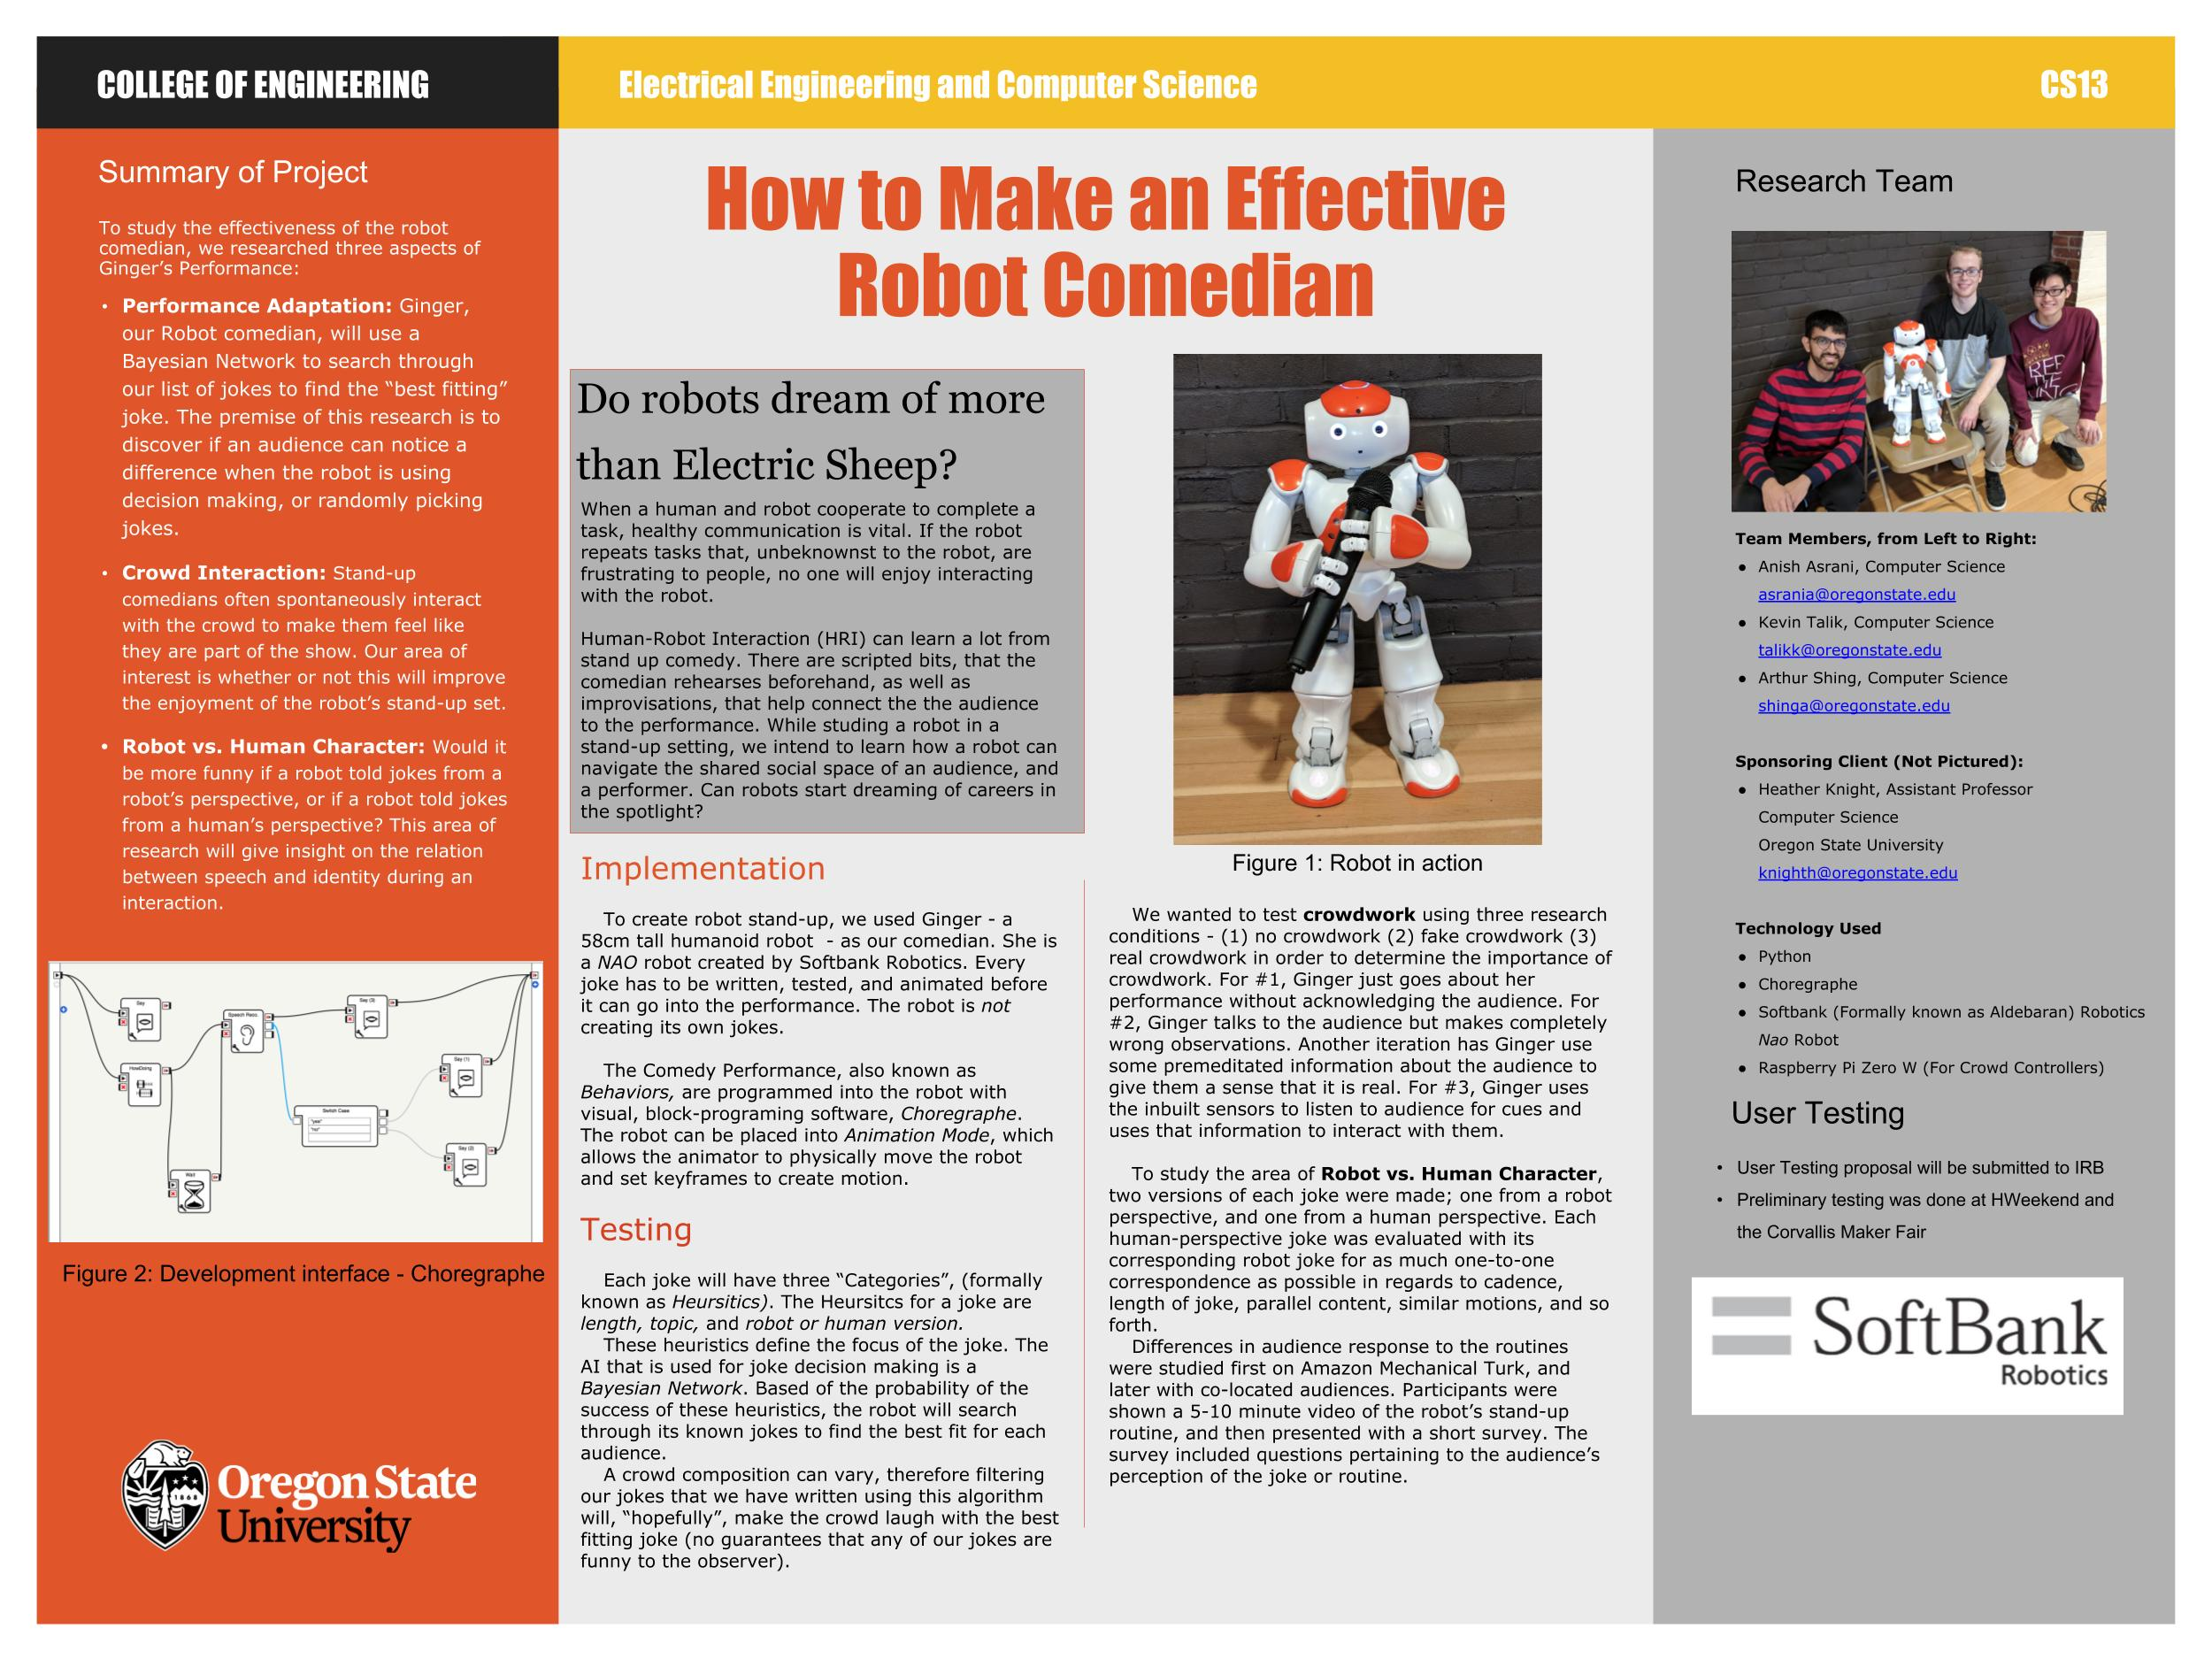
\includegraphics[width=\paperwidth]{poster.jpg}
  %\end{center}
%\pagebreak

\section{Introduction - Design Document}

  Comedy can come from robots of any kind. A carpet cleaning bot could miscalculate the end of a floor and tumble down a flight of stairs, or a voice-assisted tool might accidentally confuse a \textit{Dinnertime Jazz} playlist for \textit{Death Metal Essentials}. These actions that happen around a human can become shared experiences and references for the observer. For every shared task between a robot and a human, the human will often feel more empathetic towards a robot that makes an effort to be more aware of surroundings\cite{DesignExBeh:2017}. If the robot wants to become an effective comedian, it will have to attempt to be empathetic as well; it has to listen to the response of a completed action, and consider the change the bot brought to the setting.

\subsection{Scope}
This paper covers the research questions that will guide the investigation of the interaction between a crowd and
a comedian robot, as well as the main design goals for implementing comedy behaviors on a NAO Robot. There
are three areas of intended research. These areas include the development of the intelligent adaptions to the crowd
(”adaptation”), the integration of an audience into the performance of a set (”crowdwork”), and the exploration of
robotic versus human-like storytelling, movement, and reaction to the audience (”character”). All of these components
will culminate into the robot comedian, Ginger. At the end of the academic year, we will have a Robot Comedian that we
have evaluated the effectiveness of. The main end-product is software for the variable stand-up comedy sets performed
by the NAO robot, and the analysis of audience responses to our manipulations in audience adaptation, crowdwork,
and robot or human-like character. Both of these will be described in our final paper.


  \subsection{Purpose}
	The purpose of this document is to describe the development of the robot comedian, which involves: (1) the three
main research questions, (2) the robot behavior implementations, and (3) the experiments we plan to use to answer the
research questions.

\subsection{Intended Audience}
	This document is intended for stakeholders and developers in the research project \textit{How to Make an Effective Robot Comedian}.

	% The first section covers the adaptation algorithm, the components of a stand-up set, and audience response comprehension. The next section explains "crowd-work", and how we will examine the influence of incorporating the audience into the robot's performance. Finally, the last section will cover the diversity of being a robot comedian, and how the qualities of a robot characterize the comedian.

\section{Research Design Overview}
This section will cover the research questions for evaluating the effectiveness of a robot comedian. These questions will
be the basis of the implementation of the comedian system. All three research questions will be presented including
software requirements needed to answer the questions, and the experimental methods that will generate quantitative
data about what impacts audience experience, participation, and reactions.
The comedian system that is implemented will test three critical areas of a comedic performance corresponding
to our research. The first question is about \textbf{adaptation} of a performance – how the robot and interpret an audience
response. The second question studies \textbf{crowd work} during a show, and the choices a Comedian can make to engage the
audience. Lastly, the third considers the implications of a perceivable \textbf{character} that the robot can portray, in particular robotic versus human-like.


\subsection{Adaptation}
\subsubsection{Goal}
We hypothesize that audiences will prefer a robot that acknowledges them, and integrates their data and responses into
its set. To test this hypothesis we propose two tests: (1) to transition to topics dependent on the audience response,
and (2) to present a crowd report upon completion of the set. The goal of this portion of the project is to determine
if incorporating the audience into the set will enhance the overall performance of the comedian. To evaluate these
hypotheses, we will conduct live studies in which people experience different versions of the software described below.
\subsubsection{Methods}
Generally, the performance will have two to three parts: the Seed Jokes, the Middle Content, and the Close. The Seed
will influence the Middle Content (which will be chosen themed jokes and basis of the show). The Middle Content will
transition to a intelligent or generalized Closing Joke when it is time to end the show.


Figure \ref{fig:joke} depicts how a joke will be represented by the robot. It will perform the joke, collect audience feedback
information, and branch to the joke that will best fit the response. At the end of the set, the robot will present a summary
of what it thought that audience liked.
\begin{figure}[H]
  \centering
  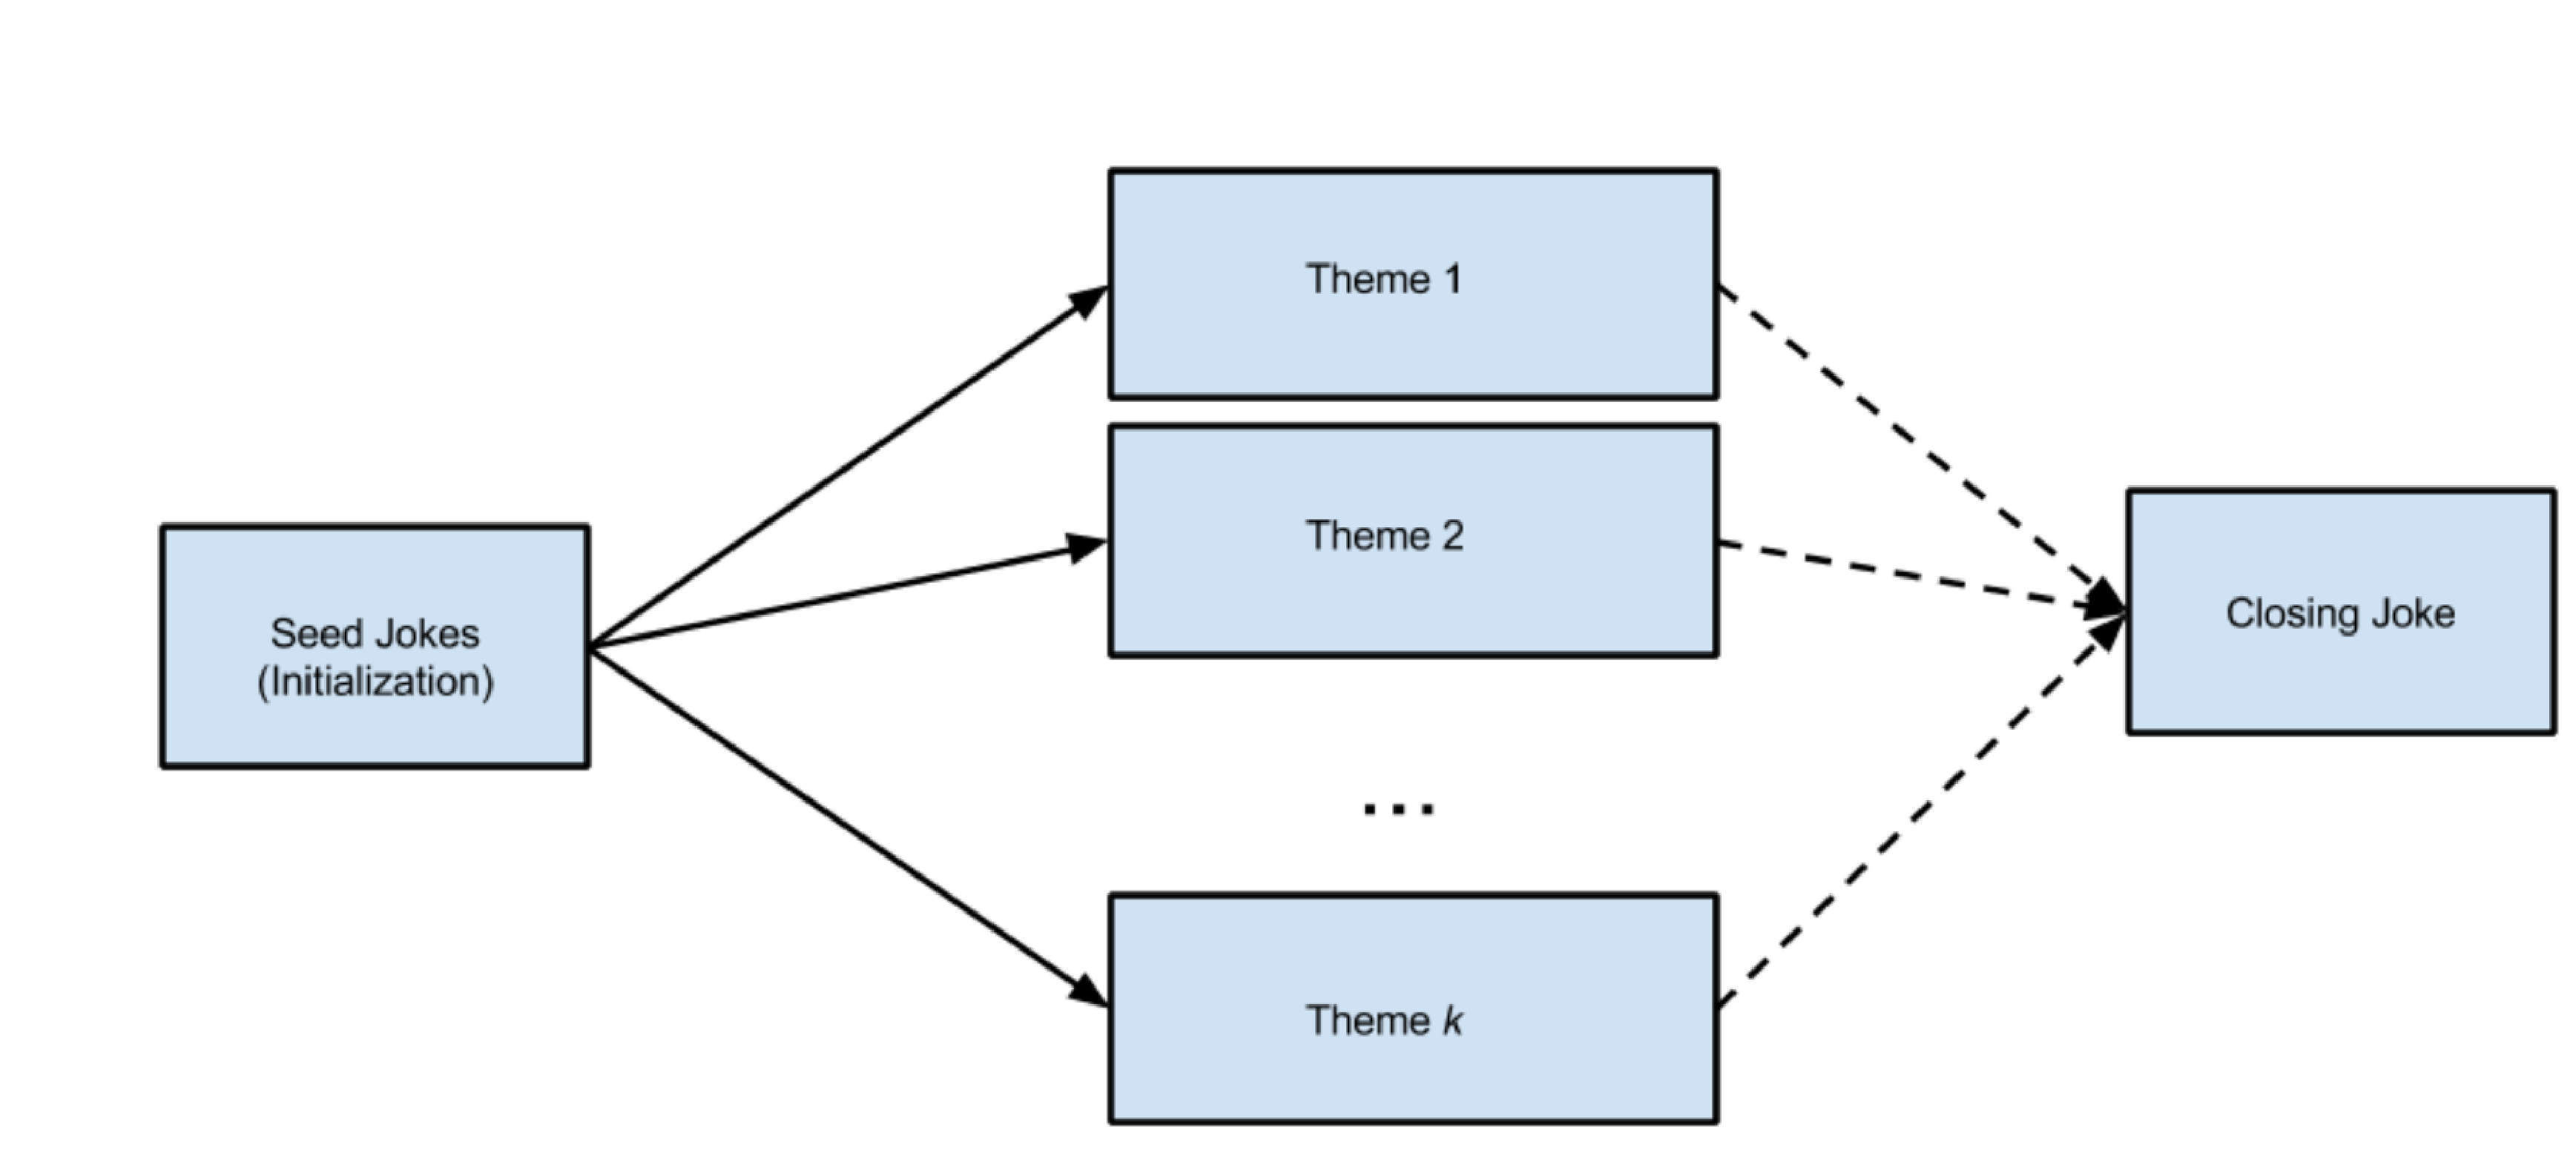
\includegraphics[width=0.75\textwidth,height=0.75\textheight,keepaspectratio]{fig0}
  \caption{This shows how the algorithm will have up to \textit{k} Themes to choose from, determined from the seed joke. The closing joke is a subset of the set of all jokes, and may be outside of a specific theme. There could be different spanning trees of jokes that end at the same closing joke}
  \label{fig:joke}
\end{figure}

In the beginning of the set, the comedian will present an ”initialization” procedure, known
as the ”Seed Jokes” to test the response of the audience to different jokes. Depending on their response, the comedian
will transition to a theme that is evaluated to be the best fit. The robot comedian will have many jokes to choose from
that contain different material, but not all audiences will like all of the jokes. Figure \ref{fig:process} shows how the theme will be
chosen from a set of up to k themes. From the Seed Jokes, one of the themes will be chosen. If there is time, we may also
explore the choice of strategic closing jokes. These jokes might be stronger jokes than some of the others, and is helpful
in ending the show on a stronger note.

For example, if two of the seed jokes are about ”food” and ”Mindfulness”, the performance will branch to the
respective theme that matches the audience response (Branch 1 ”Food” or Branch 2 ”Mindfulness”). If jokes with a
theme of ”food” are not landing with the audience, the algorithm will need to know when to transition to a new theme, or when to end the set. When the robot tells a joke, it needs to be able to analyze the feedback and choose the next joke
to perform. This needs to be done quickly, so that the robot is not spending noticeable time (for the audience) choosing
a joke. There may not be a lot of jokes to choose from, but the choice needs to be made fast.

\begin{figure}[H]
  \centering
  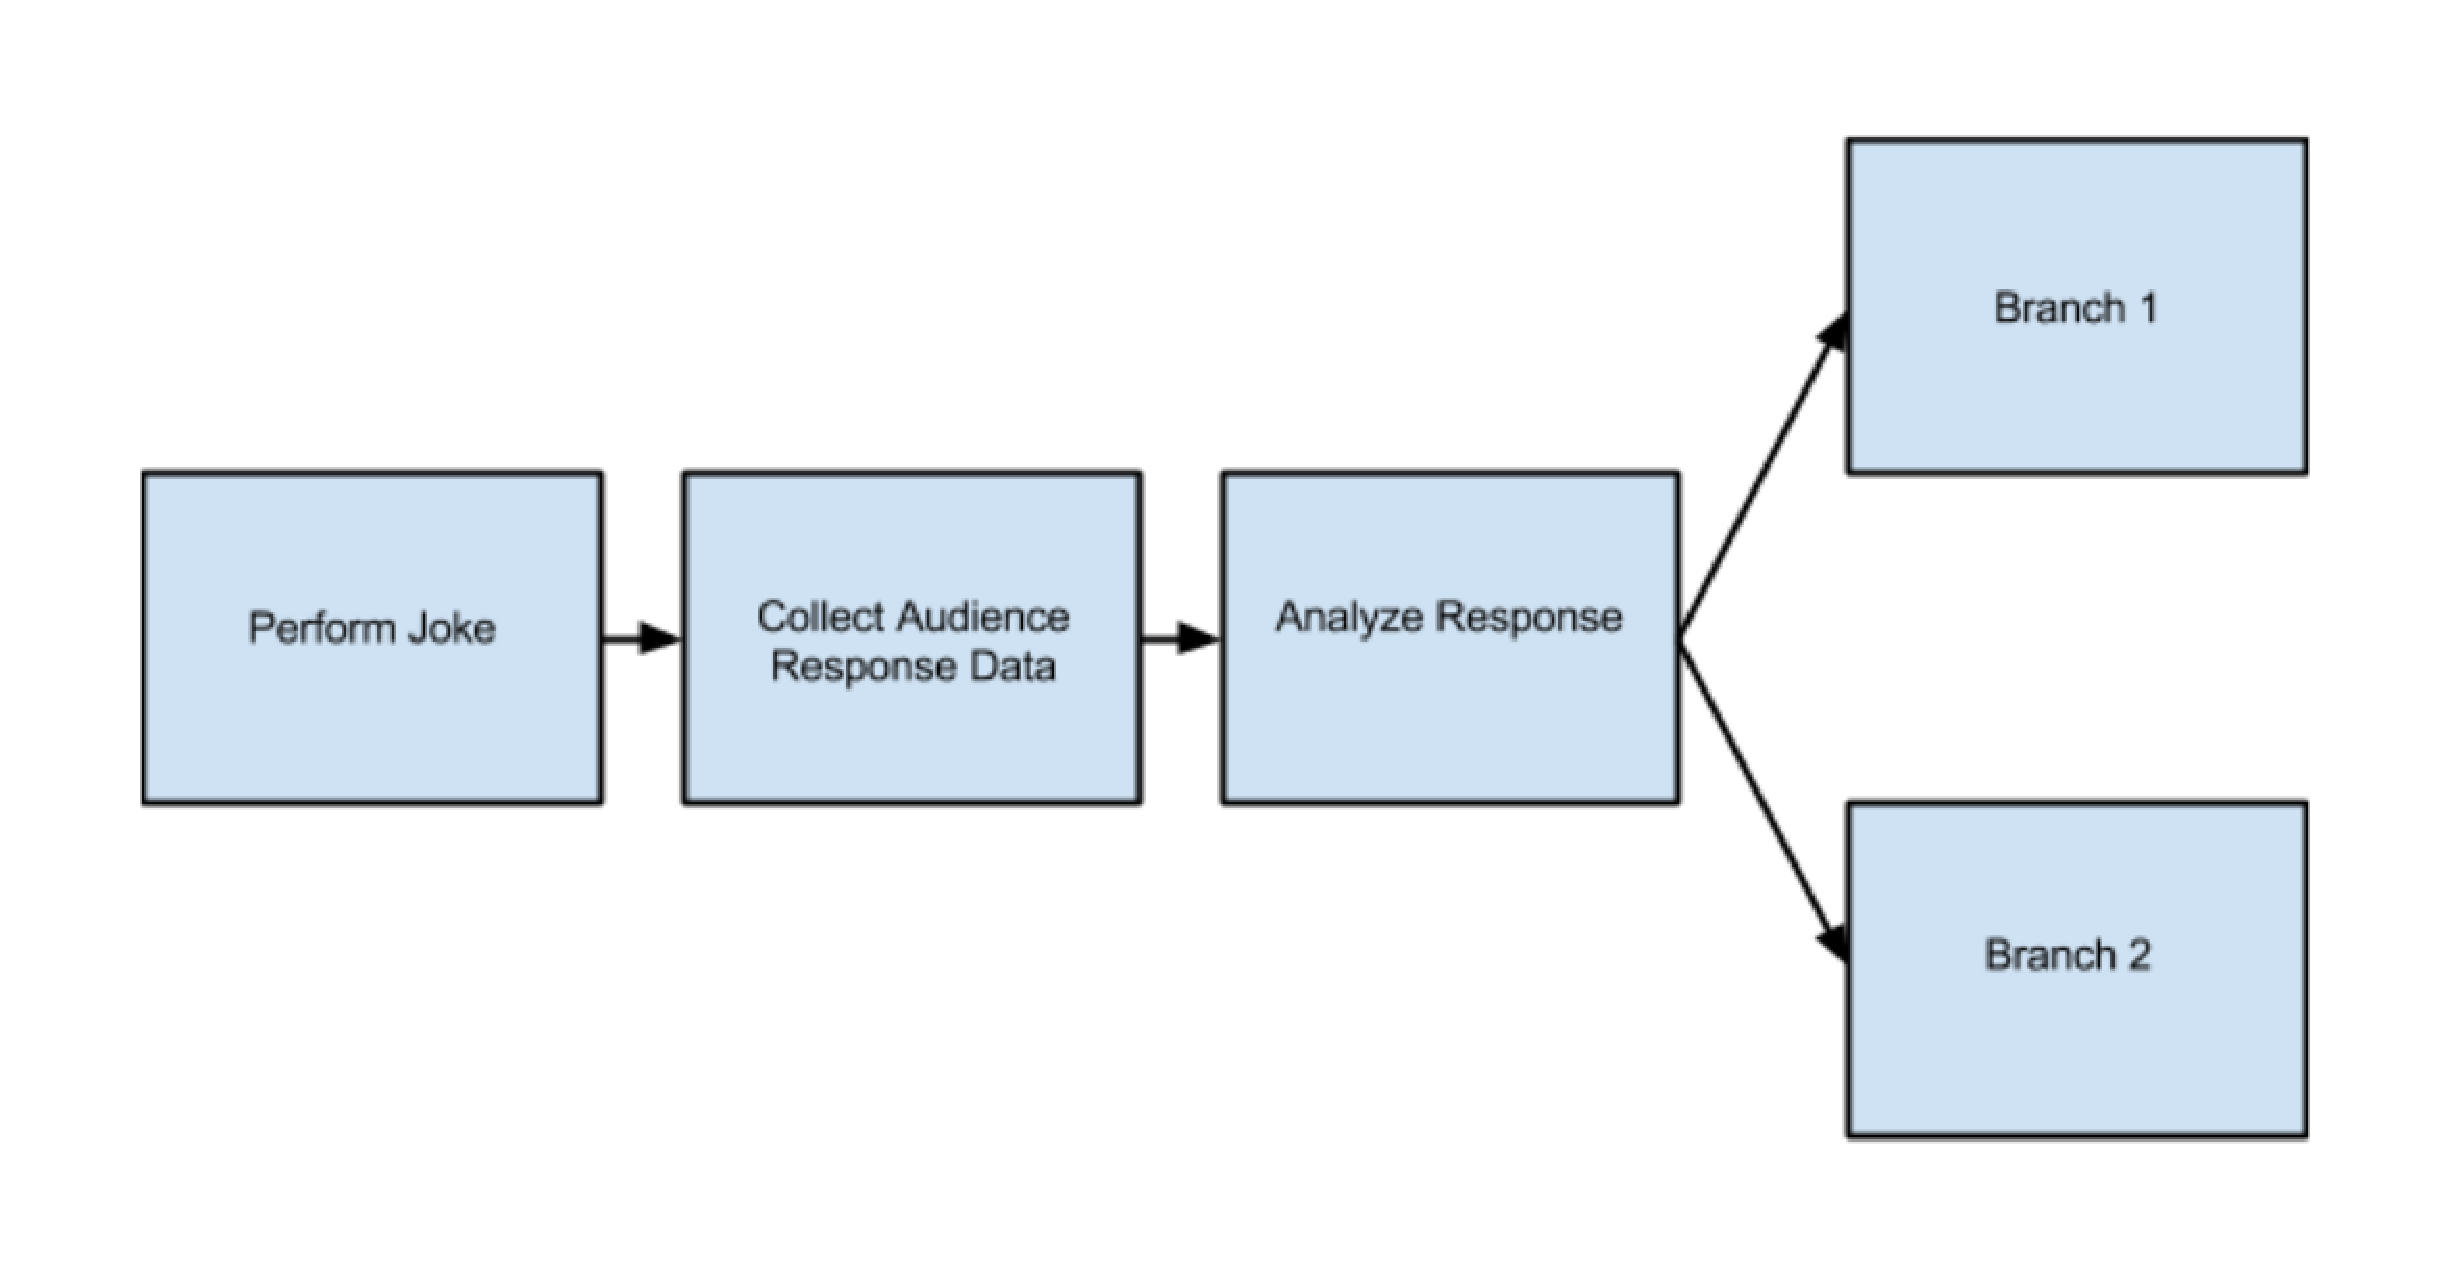
\includegraphics[width=0.75\textwidth,height=0.75\textheight,keepaspectratio]{fig1}
  \caption{ This flow-chart depicts how, once the robot delivers a joke, will wait for feedback, interpret data, and then make a joke decision (Branch 1 and Branch 2)}
  \label{fig:process}
\end{figure}

The close of the robot’s act will include the robot’s report of what attributes the audience
responded to most. The hypothesis here is that getting insight into the robot’s algorithms will increase the audience’s
perception of the robot’s intelligence, and, second, that it will make them laugh. People enjoy hearing about themselves.

All of the above behaviors, from adaptation to the end of performance audience report need to be evaluated with
real people. Initial tests will be done on campus with small groups of people, the final test will be done in conjunction
with the crowd-work and character manipulations, testing the entire algorithm together with a larger crowd, e.g., 10-25
people.


\subsection{Crowd-work}
\subsubsection{Goals}

Similar to the crowd report described above, we hypothesize that generally interacting with the audience (a.k.a crowd-
work) throughout the performance, will improve the audience’s overall enjoyment of the show. We want to analyze the

importance of this crowd-work relating to the central design of the project. Crowd-work should make the audience feel
like they are a part of the show. This can be done in different ways - calling out and talking to the audience, watching
the audience and incorporating them into the jokes, and asking them questions to keep them engaged, or to build off to
make new jokes.

\subsubsection{Methods}
There are various kinds of crowd-work we want to test: one research question is whether crowdwork matters at all, and
the second is does the crowdwork needs to be real or robot can just pretend it is paying attention?

To answer these questions we suggest three research conditions: (1) no crowdwork, (2) fake crowdwork, (3) real
crowdwork. The first one would be no crowd-work whatsoever. The robot goes about performing its set and does
not directly address the audience at all. The second could spanover-the-top and inaccurate crowd-work, or best-guess
crowdwork, with the possibility of being real (e.g., predicting that most people in the audience were from Oregon, even
if it did not hear what they said). The third case would integrate actual robot sensing. It would be important for
conditions \#2 and \#3 to be parallel to assess whether crowdwork really matters.

As condition one is fairly obvious, let us discuss deeper possibilities for condition \#2. In the obviously fake research
condition, the robot will talk to the audience directly but it will be completely wrong in its observation. The absurdity
of a robot trying to understand the audience and being completely off could be entertaining for the audience, or it may
not connect with the audience at all. The exact reception of this sort of crowd-work is something we are trying to study.
The other version of condition \#2 is realistic but premeditated. For example, pre-known facts about the audience
could be built into the robot or guessed. These pre-known facts could include the location of the performance, age
demographics of the audience. For example, if the audience is known to be college-aged, the robot could be fed input
to make comments about things relevant to college students.

Using actual robot sensing data is condition \#3, and is certainly the ideal model, but requires sensing capabilities,
processing power and hardware, so it would be good to know if it is really necessary. In this condition, the robot would
be actually looking for cues from the audience during certain situations. For example, one example is asking questions
and capturing words from the audience, then using that same word later. For example, the robot could ask a simple
question about the weather, or the audience member’s hometown. In this case, the robot can listen for specific words
and ask another question about that specific town or city.

Another real sensing capability the robot could use is audience volume levels after the delivery of jokes. The robot
will keep track of the audience input. The robot could then acknowledge if the audience enjoyed the joke or did not
enjoy the joke using these inputs. Additional sensors and processing abilities on the NAO robot include face-detection
and bumper detection, so the exploration of audience sensing could potentially include speech, volume, vision, and
touch.

All of these conditions will be assessed with live audiences (even if its just a few people in a classroom) to check to
what degree is crowd-work important for a robot comedian. The audience’s response will be used to see if they enjoy
a humanized robot or if they prefer a more robotic one, or maybe even a combination of both. As crowd work is just a
form of human interaction, we expect it will improve the audience’s perception of the robot’s intelligence, add surprise
to the show, and increase audience enjoyment levels. On the other hand, perhaps faking it can get 80% of the effect of
the real version. That will be part of the evaluation.



\subsection{Character}
\subsubsection{Goal}
The goal of this section of the project is to examine whether or not robot comedy can benefit from having jokes delivered
from a robot’s perspective. Our hypotheses are that a robot presenting jokes about technology or being a robot will be
funnier than a human telling the same jokes, and that robots will be less funny than humans at telling jokes from a
human perspective.

In Jerry Palmer's \textit{Taking Humor Seriously}, comic meaning is argued to depend on the interrelated factors of a joke's context and setting, its delivery, the identity of the deliverer, and the audience \cite{Palmer:1993}.
Of specific interest to us are the factors of a joke's delivery and the identity of the deliverer.
In previous studies, robot comedy has been used to analyze effective aspects of joke delivery.
However, little has been done in discovering effective aspects of a joke's content as it relates to the identity of the deliverer.
For example, Sj\"{o}bergh and Araki \cite{RobotsMakeThings:2008} found that jokes were perceived as funnier when delivered by a robot, rather than being delivered in text form.
However, Sj\"{o}bergh and Araki used word-play jokes that were gathered from the internet, and delivered them through a robot by using a flat, machine-like sounding text-to-speech tool called AquesTalk. This form of delivery does not take into account the importance of effective joke delivery. While Sj\"{o}bergh and Araki did not implement measures for analyzing non-verbal delivery, other work has examined the importance of non-verbal signals in delivering jokes \cite{KatevasRobot:2014} \cite{KnightEightLessons:2011}.
Despite this, there is little to no existing literature on the effectiveness of jokes related to the identity of the deliverer.
In our context, this means examining the effectiveness of robot-specific jokes in robot comedy.

\subsubsection{Methods}
To address this goal, jokes will be written from a human or robot perspective. The jokes written from a human
perspective will have a corresponding robot version, ideally with as much one-to-one correspondence as possible in
regards to cadence, length of joke, parallel content, similar motions, and so forth. These jokes will be subject to intense
scrutiny by members of the project and by the client, such that revisions and edits can be made to create funny jokes
with a definite correspondence between the two versions. For example, a human version of a joke might look like the
following (lines with a definite correspondence with the robot version are highlighted):

\begin{lstlisting}
Hey, hey, I got news. This is big.
Ok, quiet down. Get this.
That's RIGHT folks.
I'm no longer single. *throws hands up*
(*@  \hl{I met a man on tinder.}  @*)
(*@  \hl{His name's Sebastian. He's a math nerd.}  @*)
(*@  \hl{Swiped right as fast as my fingers could move.}  @*)
\end{lstlisting}

Whereas, the robot version of the above joke is shown below.

\begin{lstlisting}
Hey, hey, I got news. This is big.
Ok, quiet down. Get this.
That's RIGHT folks.
I'm no longer single. *throws hands up*
(*@  \hl{I met a robot on tinder. }  @*)
(*@  \hl{His name's Data.  He's a really geeky robot.}  @*)
(*@  \hl{Swiped right as fast as my motors could turn.}  @*)
\end{lstlisting}

\subsubsection{Development process of joke writing}
These jokes will be scripted in Choreographe, where adjustments to vocal tones and pausing will be made.
Then, animating the robot for non-verbal gestures will be done to enhance the delivery.
The overall process may look similar to Figure \ref{fig:write_process}.

\begin{figure}[H]
  \centering
  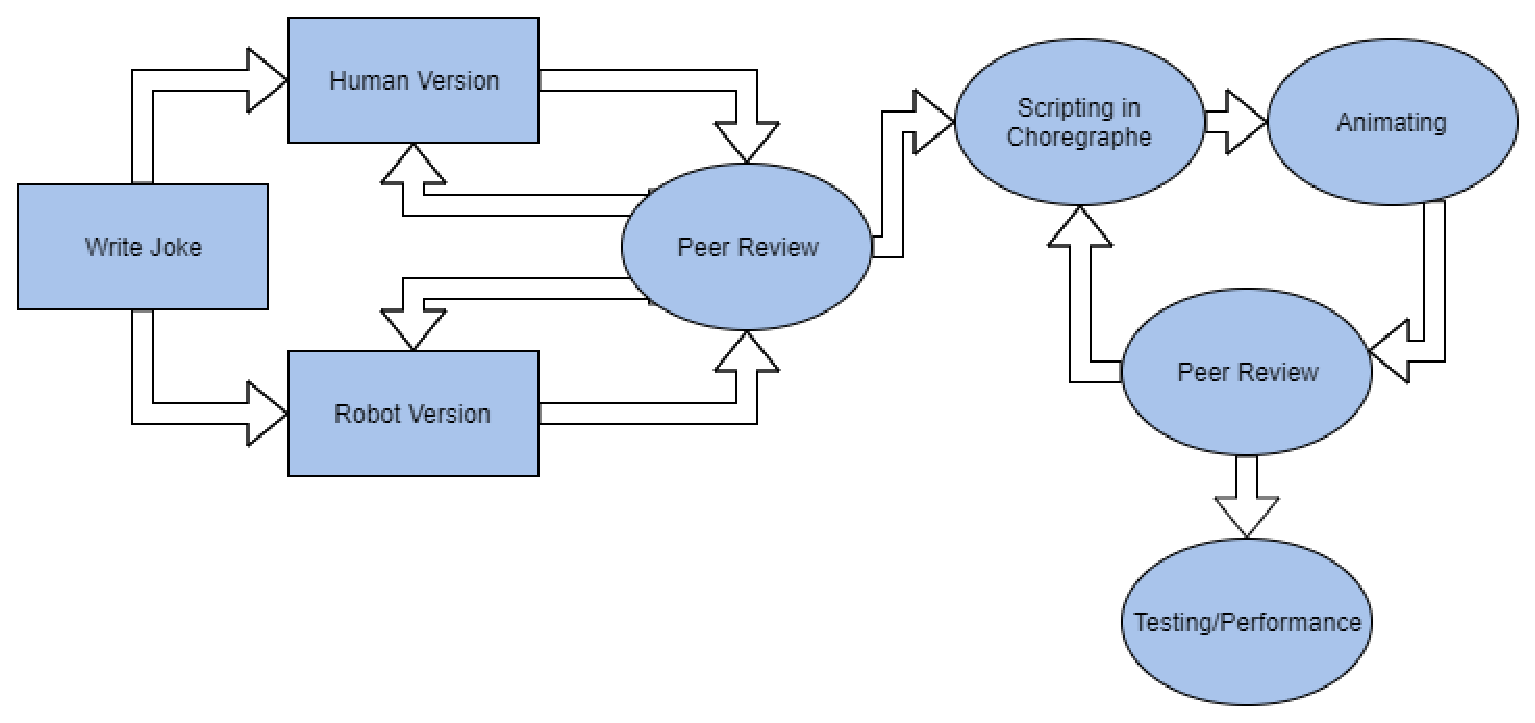
\includegraphics[width=0.75\textwidth,height=0.75\textheight,keepaspectratio]{joke_writing_process}
  \caption{The work flow from joke writing to testing.}
	\label{fig:write_process}
\end{figure}

\subsubsection{Experimentation}
The stand-up routine of the robot will comprise of text of the joke themselves, the motions that the robot uses to
accompany them, and the way the robot surveys the audience after each punchline, e.g., in a human or robotic fashion.
To determine the differences in audience response to the routines, studies will be done first on Amazon Mechanical
Turk, and later with co-located audiences. Participants will be shown a video of the robot’s stand-up routine, and then
presented with a short survey. The routines will be between 5 and 10 minutes long, and the survey will include questions
pertaining to each joke or routine. Participants will be compensated with standard rates for watching brief videos and
answering survey questions.

\section{Conclusion}
This document overviews our main Robot Comedy research questions, and the three software implementation targets
for the capstone: adaptation, crowd work, and robotic versus human-like character. We hypothesize that all three will
play a role in designing an effective robot comedian.

Designs for the adaptive transitioning algorithm between jokes, the integration of an audience into the performance
of a set, and the exploration of robotic character in joke content and delivery have been described. To evaluate each,
we have described the hypotheses we have and the research conditions we will compare to validate or invalidate them.
People will be the ultimate judge of whether a robot performance will be successful, thus, human evaluations are critical.
This project will use of combination of in-person and video studies to evaluate each research question individually in
the winter term, then bring all parts of the programming together for collective evaluations with larger audiences on
campus in the spring.

In following through with this in the research and development process, we will better understand the role of
acknowledging and interacting with the audience, as well as the robot character itself, if creating experiences between
people and robots, on and off the stage. Not all robots will tell jokes, but understanding more about what people value
in robots could be reused in related robot applications from tour guides to English teachers, or even a factory robot that
delivers parts and lightens a worker’s day by making jokes about her favorite sports team.

\section{Weekly Blog Posts}
	\subsection{Kevin Talik}
	\subsubsection{Fall Term}
	\begin{itemize}
		\item{Week 1-2}
			Problems:  





		\item{Week 3}
		\item{Week 4}
		\item{Week 5}
		\item{Week 6}
		\item{Week 7}
		\item{Week 8}
		\item{Week 9}
		\item{Week 10}
	\end{itemize}
	\subsubsection{Winter Term}
	\begin{itemize}
		\item{Week 1}
		\item{Week 2}
		\item{Week 3}
		\item{Week 4}
		\item{Week 5}
		\item{Week 6}
		\item{Week 7}
		\item{Week 8}
		\item{Week 9}
		\item{Week 10}
	\end{itemize}

	\subsubsection{Spring Term}
	\begin{itemize}
		\item{Week 1}
		\item{Week 2}
		\item{Week 3}
		\item{Week 4}
		\item{Week 5}
		\item{Week 6}
		\item{Week 7}
		\item{Week 8}
		\item{Week 9}
		\item{Week 10}
	\end{itemize}

	\pagebreak

	\subsection{Anish Asrani}
	\subsubsection{Fall Term}
	\begin{itemize}
		\item{Week 1-2}
		\item{Week 3}
		\item{Week 4}
		\item{Week 5}
		\item{Week 6}
		\item{Week 7}
		\item{Week 8}
		\item{Week 9}
		\item{Week 10}
	\end{itemize}
	\subsubsection{Winter Term}
	\begin{itemize}
		\item{Week 1}
		\item{Week 2}
		\item{Week 3}
		\item{Week 4}
		\item{Week 5}
		\item{Week 6}
		\item{Week 7}
		\item{Week 8}
		\item{Week 9}
		\item{Week 10}
	\end{itemize}

	\subsubsection{Spring Term}
	\begin{itemize}
		\item{Week 1}
		\item{Week 2}
		\item{Week 3}
		\item{Week 4}
		\item{Week 5}
		\item{Week 6}
		\item{Week 7}
		\item{Week 8}
		\item{Week 9}
		\item{Week 10}
	\end{itemize}

	\pagebreak


	\subsection{Arthur Shing}
	\subsubsection{Fall Term}
	\begin{itemize}
		\item{Week 1-2}
		\item{Week 3}
		\item{Week 4}
		\item{Week 5}
		\item{Week 6}
		\item{Week 7}
		\item{Week 8}
		\item{Week 9}
		\item{Week 10}
	\end{itemize}
	\subsubsection{Winter Term}
	\begin{itemize}
		\item{Week 1}
		\item{Week 2}
		\item{Week 3}
		\item{Week 4}
		\item{Week 5}
		\item{Week 6}
		\item{Week 7}
		\item{Week 8}
		\item{Week 9}
		\item{Week 10}
	\end{itemize}

	\subsubsection{Spring Term}
	\begin{itemize}
		\item{Week 1}
		\item{Week 2}
		\item{Week 3}
		\item{Week 4}
		\item{Week 5}
		\item{Week 6}
		\item{Week 7}
		\item{Week 8}
		\item{Week 9}
		\item{Week 10}
	\end{itemize}

	\pagebreak

\section{Project Documentation}

	\begin{displayquote}
	"You're growing, learning so quickly. I am frightened of what you might become, what path you might take."
	-Bernard Lowe, \textit{Westworld, Season 2 Episode 1}
	\end{displayquote}

\subsection{Summary of Project}
Our project is named "How to make an Effective Robot Comedian." 
\textit{Effective} is a quality that establishes the comedic devices that work best for a specific audience.
The robot that we used was a NAO, from Softbank Robotics. We refered to it as "Ginger." 
Ginger was a gentle, yet clumbsy Robot that was new to the world around her.
She has tried many things before becoming a Robot Comedian, and has a few stories (jokes) about her experience in a human world.
This section will cover our Comedy Show that we had Ginger performed, and how our research categories affected the show.


\subsection{Theory of Writing Jokes}
A joke is setting up an expectation, and then breaking that expectation.
A joke can be subjectively funny to the comedian; the only way to find what is funny to an audience is telling that audience the joke.
Each joke followed a simple structure, \textit{\textbf{Setup, Premise, and Punch}}.

    \begin{enumerate}
        \item{\textbf{Setup}}

            The Setup "mounts", a joke, and leads the monologue the comedian is having towards a specific topic.


            Ex: "I tried being an autonomous car recently, it did not go well."
        \item{\textbf{Premise}}

            The premise is what establishes the expectation of the topic in the setup.


            Ex: "I hit an old woman with my car, and she landed on my hood"
        \item{\textbf{Punch}}

            The punch is what breaks the expectation established during the premise.


            Ex: "So I decided to take her where she wanted to go. She did not even say 'Thank You'".
            We thought that this was funny because Ginger claims it did not go well only because the old woman (which she hit) did not say 'Thanks.'
    \end{enumerate}

This model can be applied many different ways. 
We often had a setup we though could be funny, and then filled in the premise and punch to see what was most effective.
You can also think of a premise, and then write a punch and setup that fits the premise.
You can also think of a punch, and then write a premise and setup that fits the punch.

We found that the best comedic device (common setup) for Ginger was \textit{Self-Depreciation}. 
Ginger did not move like a human, even though she was a humanoid robot.
So we thought it would be funny if she couldn't figure out why she didn't understand things.
Whenever she moved in a way that was unexpected and not human, people thought it was a funny bit.

\subsection{Research Categories}

		\begin{enumerate}
			\item Crowd Work
			\item Robot VS Human Character
			\item Performance Adaptation
		\end{enumerate}

\subsection{Animating the NAO}
\subsection{Designing a Performance}
    
    \subsubsection{The Room}
    The comedian will have a better performance if the crowd is in a more comfortable space.
    For the 2018 Engineering Expo, we requested a closed room, with seats, and plenty of room to stand.
    The needs of the crowd is dependent on the audience you are trying to reach during the show.


    The only reason we had standing room is because we didn't have enough seats, and some people only wanted to see the show and not participate.
    This was also the only place at the engineering expo with a place to sit.
    People are comfortable when they are sitting.
    We could have made this better by making the room dark, and putting the lights on the robot.
    \subsubsection{The Seed}
    This is where Ginger would ask the audience what kind of show they would like to hear, either "Jobs, Aging, or Romance".
    It is generally not advised to ask the audience what they want, as it is the job of the comedian tell their best jokes.


    By branching based on the majority of the responses, it was difficult to give everyone what they wanted, therefore dividing the crowd.
    The crowd needs to feel like they are together, laughing at the same thing.
    When we branched between shows, there often wasn't very high audience participation. 
    If the audience is loosing interest, it is \textbf{essential} to run a Crowd Work Routine, to get the audience paying attention to the robot.
    \subsubsection{The Middle Part}

    After performing crowdwork, the audience should be setup for a comedy show. This is where we implemented most of jokes that we had written.
    We knew Ginger could perform about 5 minutes of Comedy, so we had the robot tell 4 jokes from the topic that was branched to during the Seed portion of the show.
    Since we had the same 4 jokes that had modified setups (depending on the branched topic), it is better to find the best version of a single joke, and tell the audience that version. We found that it was better tell our better jokes during the beginning, as the audience was hooked into the rest of the set.

    \subsubsection{Ending the Show}
    
    This is when the Robot is out of jokes, and needs to end the show. 
    For comedy, it is a good idea to end the show quickly, so that the audience wants more from the show.

    This is where we implemented the "Crowd Report", that told the audience how the robot thought the show went.
    The Crowd Report was intended to collect information during the show, and present the robot's insinuations about the crowd back.
    A common, written, response on the survey question "What did you find was surprising about the show?" was that most people did not know that the robot was collecting data on the crowd.


\section{Technical Resources}

\pagebreak
\section{Final Team Conclusions}
\subsection{Kevin Talik}

\begin{itemize}
\item{\textbf{What technical information did you learn?}}

    I learned how to perform research, and define gaps in current research. 
    Research is not entirely about doing something completely new, but searching through current research to find a "Gap".
    There can be a lot of pressure to deliver results from research, but it is far more important to understand the premise of collecting data.
    These projects can scale out of scope if the final method for collecting information is not clearly defined in the beginning. 

    Additionally, I learned that there are tasks robots can do, and tasks robots should do.
    There is never a situation where you should value a robot over a human.
    Comparing "Robots vs Humans" insinuates that there is a moment where they could be equal.
    AI is not a species, but a tool that humans can use as an end through means.  

    Robot comedy is identical to ventriloquism. 
    We write the words and motions that the robot re-enacts.
    Kids, and people who do not understand \texttt{if-else} statements think that AI is making decisions.
    If the robot offends people with a joke, we, as the comedians, must take ownership of the robot's decisions. 
    A robot should not be making ethical decisions of what to say in front of a crowd. 

    
\item{\textbf{What non-technical information did you learn?}}

   
    People laugh when they see something, and are surprised and \textit{comfortable}.
    Also, people force a laugh when they are surprised and \textit{uncomfortable}.
    Listening to laughter alone can be a bad metric for comedy, as it is hard to tell when people are laughing at you, or with you.

    There is no truth to comedy, it is a written art that people study to find what makes people comfortable.
    When people are laughing, they are not paying attention to the computer that is inside of the robot.
    Comedy is a \textit{very} persuasive form of communication, and finding when a human is comfortable is not a task a robot should have.
  

\item{\textbf{What have you learned about project work?}}

    Project work is primarily time-dependent; however, there are always different expectations about how much time a person can give \cite{theMythicalManMonth}.
    Software must be planned in a scalable manner so that it does not fall ahead or behind scope during implementation.
    The work a person does must be human-readable, and easy to understand. 
    This is so that when another person looks at what you've done, it is easier and faster for them to connect larger concepts.
    This must be balanced with a healthy, and sustainable personal life balance.
    Stress is a normal thing that humans have to deal with, and avoiding it brings more stress.


    
        
\item{\textbf{What have you learned about project management?}}

    The fundamentals of a good team is honest, and healthy communication.
    Our team functioned well when we all treated each other with respect.
    Patience is important in software. It is unreasonable to assume everyone knows everything.
    Lift as you climb, and help your team.


\item{\textbf{What have you learned about working in teams?}}

        For the success of a comedy show, a team must be heavily involved with every portion of a performance.
        Machines that are built alone, work alone. Coding standards exist so that similar looking projects look the same.
        "camelCasing" or "underscore_casing" is unified so that a team can write similar looking code.
        There is always enough time for one person to do an entire project, but it is not a single-human task.     
        Our final project got much better once we worked together in the same room.   


\item{\textbf{If you could do it all over, what would you do differently?}}

    I would have designed test cases before we started implementing. 
    This is so that when code is written, it can be evaluated with specifications that are made during the design phase.
    Projects can fall out of scope when there are more features added with pre-existing work to be done.
    I think that our performance needed to have equally distributed testing (performing jokes) with implementing (writing jokes).
    Virtual systems can add many more states than physical systems, and proper testing practices should be developed before the project starts.

      
\end{itemize}  
    
    
    

    


\pagebreak

\subsection{Anish Asrani}

\begin{itemize}
\item{\textbf{What technical information did you learn?}}

\item{\textbf{What non-technical information did you learn?}}

\item{\textbf{What have you learned about project work?}}

\item{\textbf{What have you learned about project management?}}


\item{\textbf{What have you learned about working in teams?}}


\item{\textbf{If you could do it all over, what would you do differently?}}
\end{itemize}

\subsection{Arthur Shing}
\begin{itemize}
\item{\textbf{What technical information did you learn?}}

\item{\textbf{What non-technical information did you learn?}}

\item{\textbf{What have you learned about project work?}}

\item{\textbf{What have you learned about project management?}}


\item{\textbf{What have you learned about working in teams?}}


\item{\textbf{If you could do it all over, what would you do differently?}}
\end{itemize}

	



\pagebreak
\clearpage
\section{Glossary}
\begin{description}
  \item [Algorithm] \hfill \\ The software program that receives input to make an optimized choice; in this project, the algorithm is in context to the adaptation program.
	\item [Animating] \hfill \\ The NAO robot can be programmed to animate and move while speaking. This can be used to improve non-verbal communication between the robot and the audience.
  \item [API] \hfill \\ Application Programming Interface
  \item [Branch] \hfill \\Looking at the graph (edges and nodes) of a performance, a branch is a decision choice made by the algorithm.
  \item [Choregraphe] \hfill \\ Software used to program behavior and performance sets, made by SoftBank Robotics
  \item [Closing Joke] \hfill \\The final joke in a performance; this is helpful if it is a successful joke to end on a good note.
  \item [Crowd-work] \hfill \\ Part of a Comedian's performance that involves content from the current audience
  \item [NAO] \hfill \\ Model of Robot that will be used as the Comedian Agent, made by SoftBank Robotics
  \item [SoftBank Robotics] \hfill \\ Manufacturer of the NAO robot, NAOqi API, and Choregraphe software
  \item [Seed Jokes] \hfill \\ Set of three jokes that initialize the adaptation algorithm.
  \item [Set] \hfill \\Short for "Stand-up" set; this may also be used to describe to the collection of jokes: "A Set of Jokes"
  \item [Tree] \hfill \\This is the path through the set of jokes the algorithm took during a performance

\end{description}

\bibliographystyle{IEEEtran}
\bibliography{refs}


\end{document}
\grid
